% !TeX spellcheck = de_CH
% !TeX encoding = UTF-8
% !TeX root = ../presentation.tex

\section{Spinodale Entmischung}

\begin{frame}{Spinodale Entmischung}
\begin{itemize}
\item Bezeichnet die Trennung von Mischungen zweier Stoffe in
koexistierende Phasen
\item $\Rightarrow$ Öl-Essig-Mischung (Salatsauce)
\end{itemize}
\end{frame}

\begin{frame}{Beispiel}
\begin{figure}
\centering
\foreach \n [count=\xi] \i in {0,5,10,15,25,50,80,130,300}{
\begin{subfigure}{0.18\textwidth}
\centering
\uncover<\xi->{
\includegraphics[width=\textwidth]{images/ch_sim/\i.pdf}
\vspace{-0.5cm}
}
\caption{$t = \i\,\tau$}
\end{subfigure}
}
\begin{subfigure}{0.18\textwidth}
\centering
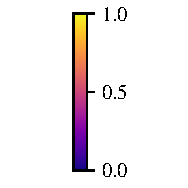
\includegraphics[width=\textwidth]{images/colorbar}
\caption{Farbskala}
\end{subfigure}
\end{figure}
\end{frame}


\begin{frame}{Beispiel}
\begin{figure}
\centering
\foreach \n [count=\xi] \i in {130,300,1500,70000}{
\begin{subfigure}{0.18\textwidth}
\centering
\uncover<\xi->{
\includegraphics[width=\textwidth]{images/ch_sim/\i.pdf}
\vspace{-0.5cm}
}
\caption{$t = \i\,\tau$}
\end{subfigure}
}
\begin{subfigure}{0.18\textwidth}
\centering
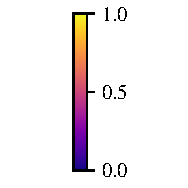
\includegraphics[width=\textwidth]{images/colorbar}
\caption{Farbskala}
\end{subfigure}
\end{figure}
\end{frame}

